%  LaTeX support: latex@mdpi.com 
%  In case you need support, please attach all files that are necessary for compiling as well as the log file, and specify the details of your LaTeX setup (which operating system and LaTeX version / tools you are using).

%=================================================================
\documentclass[data,datadescriptor,submit,moreauthors,pdftex]{Definitions/mdpi} 

\usepackage{enumitem}
\hypersetup{
    colorlinks,
    linkcolor={red!50!black},
    citecolor={blue!50!black},
    urlcolor={blue!80!black},
    pdfborder={0 0 0}
}
\usepackage{hyperref}
\usepackage{multirow}
\usepackage{pgfplots}
\usepackage{float}
\usepackage{amssymb}
\usepackage{cleveref}
\usepackage[english]{babel}
\usepackage[utf8]{inputenc}
% \usepackage[T1]{fontenc}
% \usepackage{changepage}
\usepackage{longtable}
\usepackage{tabularx}
\usepackage{listings}
\lstdefinelanguage[]{spq}
{
    morecomment=[s][\color{olive}\bf]{<}{>},
    basicstyle = \ttfamily\footnotesize,
    commentstyle=\color{green},
    keywordstyle=\color{brown},
    morecomment=[s][\color{blue}\bf]{?}{\ },
    morekeywords={BASE,PREFIX,SELECT,DISTINCT,CONSTRUCT,DESCRIBE,ASK,%
    FROM,NAMED,WHERE,ORDER,BY,ASC,DESC,LIMIT,OFFSET,OPTIONAL,%
    GRAPH,UNION,FILTER,a,STR,LANG,LANGMATCHES,DATATYPE,BOUND,%
    isIRI,isURI,isBLANK,isLITERAL,REGEX,true,false},%
    sensitive=false,%
    % morecomment=[l]\#,%
    morestring=[d][\color{red}]',%
    morestring=[d]"%
}
% \usepackage[showframe=true]{geometry}
%

\newcommand{\textttt}[1] {\texttt{\footnotesize#1}}
\newcommand{\te}[1] {\texttt{\footnotesize#1}}
\newcommand{\h} {\hphantom ~ }
% \newcommand{\textttt}[1] {\mbox{\texttt{\footnotesize#1}}}
% \newcommand{\textttt}[1] {
% \begin{verbatim} #1 \end{verbatim}
% }
\linespread{1}
\pgfplotsset{compat=1.5}
\pgfplotsset
{
	width=0.5\textwidth,
	x tick label style={/pgf/number format/1000 sep=},
  enlarge x limits = 0.0,
  ymajorgrids=true,
	major tick style={draw=none},
  ymin = 0.0,
	every axis/.append style={
		every x tick label/.append style={font=\tiny},
    every y tick label/.append style={font=\tiny},
    every axis label/.append style={font=\small},
    height=37mm,
    width=37mm,
    title style={at={(0.5,0.90)}, font=\normalfont},
    xticklabel style={yshift=4pt}
	}
}
\usepackage{booktabs}
% If you would like to post an early version of this manuscript as a preprint, you may use preprint as the journal and change 'submit' to 'accept'. The document class line would be, e.g., \documentclass[preprints,article,accept,moreauthors,pdftex]{mdpi}. This is especially recommended for submission to arXiv, where line numbers should be removed before posting. For preprints.org, the editorial staff will make this change immediately prior to posting.

%--------------------
% Class Options:
%--------------------
%----------
% journal
%----------
% Choose between the following MDPI journals:
% acoustics, actuators, addictions, admsci, aerospace, agriculture, agriengineering, agronomy, algorithms, animals, antibiotics, antibodies, antioxidants, applsci, arts, asc, asi, atmosphere, atoms, axioms, batteries, bdcc, behavsci , beverages, bioengineering, biology, biomedicines, biomimetics, biomolecules, biosensors, brainsci , buildings, cancers, carbon , catalysts, cells, ceramics, challenges, chemengineering, chemistry, chemosensors, children, cleantechnol, climate, clockssleep, cmd, coatings, colloids, computation, computers, condensedmatter, cosmetics, cryptography, crystals, dairy, data, dentistry, designs , diagnostics, diseases, diversity, drones, econometrics, economies, education, ejihpe, electrochem, electronics, energies, entropy, environments, epigenomes, est, fermentation, fibers, fire, fishes, fluids, foods, forecasting, forests, fractalfract, futureinternet, futurephys, galaxies, games, gastrointestdisord, gels, genealogy, genes, geohazards, geosciences, geriatrics, hazardousmatters, healthcare, heritage, highthroughput, horticulturae, humanities, hydrology, ijerph, ijfs, ijgi, ijms, ijns, ijtpp, informatics, information, infrastructures, inorganics, insects, instruments, inventions, iot, j, jcdd, jcm, jcp, jcs, jdb, jfb, jfmk, jimaging, jintelligence, jlpea, jmmp, jmse, jnt, jof, joitmc, jpm, jrfm, jsan, land, languages, laws, life, literature, logistics, lubricants, machines, magnetochemistry, make, marinedrugs, materials, mathematics, mca, medicina, medicines, medsci, membranes, metabolites, metals, microarrays, micromachines, microorganisms, minerals, modelling, molbank, molecules, mps, mti, nanomaterials, ncrna, neuroglia, nitrogen, notspecified, nutrients, ohbm, optics, particles, pathogens, pharmaceuticals, pharmaceutics, pharmacy, philosophies, photonics, physics, plants, plasma, polymers, polysaccharides, preprints , proceedings, processes, proteomes, psych, publications, quantumrep, quaternary, qubs, reactions, recycling, religions, remotesensing, reports, resources, risks, robotics, safety, sci, scipharm, sensors, separations, sexes, signals, sinusitis, smartcities, sna, societies, socsci, soilsystems, sports, standards, stats, surfaces, surgeries, sustainability, symmetry, systems, technologies, test, toxics, toxins, tropicalmed, universe, urbansci, vaccines, vehicles, vetsci, vibration, viruses, vision, water, wem, wevj

%---------
% article
%---------
% The default type of manuscript is "article", but can be replaced by: 
% abstract, addendum, article, benchmark, book, bookreview, briefreport, casereport, changes, comment, commentary, communication, conceptpaper, conferenceproceedings, correction, conferencereport, expressionofconcern, extendedabstract, meetingreport, creative, datadescriptor, discussion, editorial, essay, erratum, hypothesis, interestingimages, letter, meetingreport, newbookreceived, obituary, opinion, projectreport, reply, retraction, review, perspective, protocol, shortnote, supfile, technicalnote, viewpoint
% supfile = supplementary materials

%----------
% submit
%----------
% The class option "submit" will be changed to "accept" by the Editorial Office when the paper is accepted. This will only make changes to the frontpage (e.g., the logo of the journal will get visible), the headings, and the copyright information. Also, line numbering will be removed. Journal info and pagination for accepted papers will also be assigned by the Editorial Office.

%------------------
% moreauthors
%------------------
% If there is only one author the class option oneauthor should be used. Otherwise use the class option moreauthors.

%---------
% pdftex
%---------
% The option pdftex is for use with pdfLaTeX. If eps figures are used, remove the option pdftex and use LaTeX and dvi2pdf.

%=================================================================
\firstpage{1} 
\makeatletter 
\setcounter{page}{\@firstpage} 
\makeatother
\pubvolume{xx}
\issuenum{1}
\articlenumber{5}
\pubyear{2019}
\copyrightyear{2019}
%\externaleditor{Academic Editor: name}
\history{Received: date; Accepted: date; Published: date}
%\updates{yes} % If there is an update available, un-comment this line

%% MDPI internal command: uncomment if new journal that already uses continuous page numbers 
%\continuouspages{yes}

%------------------------------------------------------------------
% The following line should be uncommented if the LaTeX file is uploaded to arXiv.org
%\pdfoutput=1

%=================================================================
% Add packages and commands here. The following packages are loaded in our class file: fontenc, calc, indentfirst, fancyhdr, graphicx, lastpage, ifthen, lineno, float, amsmath, setspace, enumitem, mathpazo, booktabs, titlesec, etoolbox, amsthm, hyphenat, natbib, hyperref, footmisc, geometry, caption, url, mdframed, tabto, soul, multirow, microtype, tikz

%=================================================================
%% Please use the following mathematics environments: Theorem, Lemma, Corollary, Proposition, Characterization, Property, Problem, Example, ExamplesandDefinitions, Hypothesis, Remark, Definition, Notation, Assumption
%% For proofs, please use the proof environment (the amsthm package is loaded by the MDPI class).

%=================================================================
% Full title of the paper (Capitalized)
\Title{LOSD: A Linked Open Social Dataset for Scientific Benchmarking}

% Author Orchid ID: enter ID or remove command
\newcommand{\orcidauthorA}{https://orcid.org/0000-0002-9699-629X} % Add \orcidA{} behind the author's name
\newcommand{\orcidauthorB}{https://orcid.org/0000-0002-5399-5860} % Add \orcidB{} behind the author's name

% Authors, for the paper (add full first names)
\Author{Renato Fabbri $^{1}$*\orcidA{} and Osvaldo N. Oliveira Junior $^{2}$\orcidB{}}

% Authors, for metadata in PDF
\AuthorNames{Renato Fabbri, Osvaldo Novais de Oliveira Junior}

% Affiliations / Addresses (Add [1] after \address if there is only one affiliation.)
\address{%
$^{1}$ \quad Institute of Mathematical and Computer Sciences, University of São Paulo (ICMC/USP), São Carlos, Brazil; renato.fabbri@gmail.com\\
$^{2}$ \quad São Carlos Institute of Physics, University of São Paulo (IFSC/USP), São Carlos, Brazil; chu@ifsc.usp.br}

% Contact information of the corresponding author
\corres{Correspondence: renato.fabbri@gmail.com}

% Current address and/or shared authorship
% \firstnote{Current address: Affiliation 3} 
% \secondnote{These authors contributed equally to this work.}
% The commands \thirdnote{} till \eighthnote{} are available for further notes

%\simplesumm{} % Simple summary

%\conference{} % An extended version of a conference paper

% Abstract (Do not insert blank lines, i.e. \\) 
\abstract{
The fields of social network analysis and complex networks
are widely researched.
In fact, a myriad of results have been reported which are based in
diverse data, most often not accessible to researchers other than the publishing authors.
In order to provide the scientific community a common repertoire,
this work presents an open dataset with diverse provenance of 
human social online networking.
Current data was obtained in 2013-16 from well-known online social networking platforms:
Facebook, Twitter, IRC, Email.
Data from ParticipaBR, AA, and Cidade Democrática are also supplied as samples of less known instances.
The linked data representation was adopted in order to
comply with current best practices, homogenize access, facilitate discovery
and analyzes which integrate third party and provided data.
Futhermore, the method for obtaing and making the data available is potentially novel,
and may be of use for other research groups.
This document presents a description, usage remarks and overall statistics of the dataset,
which should favor subsequent work in complex and social networks and enhancements to the dataset.
}

% Keywords
\keyword{social networks; complex networks; linked data; semantic web; big data; benchmark data; Facebook; Twitter; irc; email}

%%%%%%%%%%%%%%%%%%%%%%%%%%%%%%%%%%%%%%%%%%
% Only for the journal Data:
\dataset{https://rfabbri.linked.data.world/d/linked-open-social-data/}

\datasetlicense{CC0}

\begin{document}
\section{Summary}
The research on human social and complex networks often
rely on data that express real phenomena~\cite{c1,c2,c3}.
Such data is regularly not made publicly available,
which hinders validation of the results
and does not favor subsequent work.
Furthermore, there is a lack of open datasets for benchmarking results
related to complex and social networks,
yielding diverse results from poorly related sources.
Social networks linked datasets are currently most often restricted to a specific platform or express statistics of social networks, as described in Section~\ref{srel}.
This work presents 
a dataset named LOSD (Linked Open Social Data)
that has been achieved by linking social data derived from diverse
provenance, namely: Facebook, Twitter, IRC, Email groups, ParticipaBR, Cidade Democrática, and AA.
Such data may be of use as a common and public repertoire for scientific
research involving complex networks, specially if social networks and textual content are pinpointed.
In fact, the data has already been used in scientific research~\cite{stab,thesis} (CNPq grant 140860/2013-4),
and should be further used e.g. in researching complex networks and data visualization (FAPESP grant 2017/05838-3)
which relies on networks enriched by textual data and on dynamic (or time-evolving) networks.
Data collection was performed by a potentially innovative method which places the researcher
at the core of data collection, and keeps the resources (e.g. code, data, documents) open,
in order to ammeliorate ethical issues involved in studying human social systems.

This paper is organized as follows. Next subsection briefly discusses related work.
Section~\ref{materials} describes the data currently available.
Section~\ref{methods} describes the methods used for data gathering, translation into RDF linked data, and the synthesis of auxiliary structures.
Section~\ref{usage} holds directions for using the data. 

\subsection{Related work}\label{srel}
Most available datasets on human social networks rely only on one source (e.g.~\cite{nat,fb1}),
on specialized communities such as related to research or movies (e.g.~\cite{s1},
or present only statistics about social networks, and not the data that yields the networks (e.g.~\cite{st1}.
Linked human social network data is scarcely found in the scientific community.
In~\cite{foaf1}, the authors presented a set of tools to obtain linked social data available in the public data cloud, and made available a dataset from the Advogato platform,
dedicated to free software developers linked by trust relatioships.
There are various datasets which makes available data obtained from Twitter (e.g.~\cite{tw1,tw2}),
most often with a specific focus (users, retweets, hashtags, etc)
and not presented to the scientific community by means of a research article.
The datasets which are most closely related to LOSD are KONECT~\cite{konect},
SNAP Datasets~\cite{snapnets}, the Network Repository~\cite{nr}, and ICON~\cite{icon}.
None of them are (RDF) linked data but express the networks in formats specialized for networks.
In total, these datasets make available thousands of social networks, from diverse provenance and of various types (e.g. simple, directed, weighted, bipartite, temporal networks).
Compared to LOSD, KONECT, SNAP, Network Repository, and ICON are complementary, providing a further diversity of networks, but only as simplified data, i.e. in specialized formats, most often expressed as columns of node ids that are connected and metadata (such as timestaps for temporal networks).
In summary, no linked human social network dataset presented to the
scientific community containts the diverse provenance used in LOSD,
or provides such a wide range of metadata,
potentially because researchers did not have the means to acquire and
share the data as described in Section~\ref{acq},
and because linked data standards are (still) not widely adopted in 
every research domain.

\section{Data Description}\label{materials}
\subsection{Data outline}\label{outline}
% scripts/percolationUse2.py
The database consists of 31,996,740 triples, 3,030,433 network links yield by main interactions or relations, 350,284 participants and 245,194,377 characters. Among all snapshots, 63 are ego snapshots, 54 are group snapshots; 50 have interaction edges, 89 have friendship edges; 43 have text content from messages.
Section~\ref{queries} holds the queries used to obtain such data.
This section describes de data in LOSD in very brief terms.
The Supplementary document is provided for further information about the dataset.

\noindent Data was gathered from:
\begin{itemize}
    \item public APIs (Twitter, Email);
    \item public logs (IRC and AA);
    \item Netvizz software~\cite{netvizz} and subsequent donation by users (Facebook);
    \item donation by system administrators (AA, ParticipaBR, Cidade Democr\'atica).
\end{itemize}

\subsection{Snapshots}
Of central importance to the presented dataset is the concept of a snapshot.
A snapshot is herein a set of data gathered together, at a contiguous time
unit.
Examples: the first 20 thousand email messages of an email list
comprises a snapshot; the tweets from the MAMA music event is a
snapshot; the friendship, interaction and posts structures of a facebook
group, prospected at the same time, is a snapshot.
Table~\ref{tsnap} holds the number of snapshots from each provenance in LOSD.

\begin{table*}[h!]
\begin{center}
\caption{Number of snapshots from each provenance. Every snapshot is a \texttt{po:Snapshot}; there are three types of the \texttt{po:AASnapshot} class.}
\begin{tabular}{| l | c |}\hline
\textbf{snapshot provenance} & \textbf{number of snapshots} \\\hline\hline\hline
http://purl.org/socialparticipation/po/Snapshot & 117 \\\hline
\end{tabular}\end{center}
\end{table*}

\subsection{Facebook data}
Friendship ego networks (networks whose nodes represent friends of a user and links represent friendships)
were donated from individual users in 2013 and 2014.
Friendship and interaction networks from groups were gathered from
groups where the first author was a participant.
Additionally, some groups have post texts along some metadata, such as
the number of likes.

\subsection{Twitter data}
Tweets were gathered through the Twitter streaming public API.
Each snapshot is unified by a distinct hashtag.
Network links are canonically yield by retweets,
but replies and user mentions are also kept in the database.
LOSD kept the main data fields returned by Twitter API, such as creation date, text, and hashtags.

\subsection{IRC data}
Public IRC (Internet Relay Chat) logs were used to obtain IRC snapshots.
LOSD holds records of relations yield by directed messages and
mentions and the text related to each message.

\subsection{Email data}
Email snapshots refer to individual email lists.
All messages were obtained from the Gmane public email archive~\cite{gmane}.
Each message has the original text and the text without some of the lines
from previous messages or that are software code or author signature.
Most importantly, each message instance holds the ID of the message it is
a reply to, if any, which enables the achievement of canonical interaction networks~\cite{bird,stab}.

\subsection{ParticipaBR data}
ParticipaBR is a Brazilian federal platform for social participation,
the most important platform from the myriad of social participation platforms
that were available in 2011-2018~\cite{spbr}.
Texts are derived from blog posts and networks may be obtained from
both friendship and interaction criteria.

\subsection{Cidade Democrática data}
Cidade Democrática is a Brazilian civil society social participation portal.
Data gathered is complex in the number of types of instances as noticeable in the Supplementary document.

\subsection{AA data}
AA (Algorithmic Autoregulation~\cite{aa,aa2}) is a software to keep track of dedications by sharing sentences about ongoing work and testifying about their quality.
The data was gathered from different versions of the system and from an IRC
log.
 
 
\section{Methods}\label{methods}
LOSD is expressed as linked data through RDF
and is ontologicaly described through the
data-driven ontology synthesis method presented in Section~\ref{ont}.

\subsection{Data acquisition}\label{acq}
Research involving human subjects raise well-known ethical issues,
although ethical regulation for (non-medical) research in social systems is not always endorsed by scientists~\cite{eth}.
Furthermore, the online social networking platforms often restrict access
to the data and user may consider illegal the use of their data through web crowlers~\cite{ile1,ile2,ile3}.
Although Twitter and GMANE (email) data is available through public APIs,
the other sources are more problematic.
In this context, research using data, e.g. from Facebook, is precarious
if not prohibited.
We reached a potential solution to this issue through continuated research with
collaborators in the fields of phylosophy, social sciences, antropology and psychology.
The conceptual framework is presented in~\cite{antphy,antphy2}, and in essence
consists in researching first the social networks related to the researchers,
and keeping the procedures, data, algorithms and results publicly available.
These practices enabled collecting and sharing the data in LOSD,
and was called ``Anthropological Physics'' because it relies in the
etnographic tecnique of investigating the social structures
by studying the researcher, as to ammeliorate the ethical issues
(not to be confused e.g. with ``virtual ethnography''~\cite{veth}).
Accordingly, aside from the data acquired from Twitter, all data in LOSD
was gathered from social instances where the first author is a participant.
For example, all Facebook ego networks were donated to the first author by
users which know him and were interested in his research and intervention on the networks,
and all email and Facebook groups data was obtained from groups where the first author is a member.

Facebook data was obtained through the Netvizz software~\cite{netviz},
Facebook allowed downloading friendships and interaction data as available in LOSD.
Data from Twitter was obtained through the Twitter streamming API.
Data From IRC was obtained through bots that kept logs of the messages.
Email data was obtained through the GMANE public API.
Data from ParticipaBR, Cidade Democrática, and AA was obtained through contact
of the researcher with the developers of the platforms.

\subsection{Linked open data}
Linked data refers to data published in the web in such a way that it is
machine readable and conforms to a set of best practices.
The yielded web of data is composed of documents on the web
such as the web of HTML documents.
In practice, the publication of linked data can me summarized
by 1) the use of RDF and 2) the use of RDF
links to interlink data from different sources~\cite{ld1,ld2}.
The web is expected to be interconnected and to
grow by the systematic application of four
steps~\cite{lee1}:
\begin{itemize}
    \item Use URIs to identify things~\cite{uri}.
    \item Use HTTP URIs.
    \item Provide useful information when a URI is accessed via HTTP.
    \item Provide other URIs in the description of resources so human
        and machine agents can perform discovery.
\end{itemize}

The Linked Open Data~\cite{lod} cloud is a constantly growing cloud of data,
the global data space, which is usually
conceived as centered around the DBPedia, a linked data representation
of data from Wikipedia~\cite{dbpedia0,dbpedia},
and sometimes called the Giant Global Graph (GGG, akin to the WWW).

\subsection{RDF}
The Resource Description Framework (RDF), a W3C
recommendation, is a model for data
interchange.
It is based on the idea of making statements about resources in the form
of triples, i.e. expressions in the form ``subject - predicate -
object''.
RDF can be serialized in several file formats, including RDF/XML,
Turtle and Manchester, which all, in essence, represent a labeled and
directed multi-graph.
RDF may be stored in a type of database called a triplestore.~\cite{rdf}

As an example of an RDF statement, the following triple in the Turtle
format asserts that ``the paper has color white'':\\
\texttt{http://example.org/Thing\#Paper http://example.org/hasColor\\
http://example.org/Color\#White .}

\subsection{RDFS and OWL ontologies}\label{sont}
One of the most important notions of the semantic web is that of an ontology~\cite{ont}.
An ontology, in this context, is a formalized conceptualization, comprised by
concepts and relations between the concepts and between the relations themselves.
In current semantic web, most simple ontologies are written using the RDFS protocol,
by which one can specify, among other things~\cite{rdfs}:
\begin{itemize}
  \item concepts;
  \item properties, which are concepts that are used as predicates and thus relate concepts;
  \item special relations between concepts that state that one concept is more general than the other\footnote{This
          kind of relation is called hypernymy. Examples: mammal is a hypernym of monkey, drink is a hypernym of beer.};
  \item the subjects and objects that can occurs in a triple where a specific property is a predicate.
\end{itemize}

One can also write an ontology using the OWL protocol,
with which all the expressive capabilities of RDFS are
available, but one can also, among other things~\cite{ont}:
\begin{itemize}
  \item state ``property axioms'', i.e. specify if a property is e.g. reflexive or transitive;
  \item state ``class restrictions'', i.e. specify if a class instance e.g. necessarily holds a relation to another class instance or data.
\end{itemize}
OWL has a richer vocabulary than RDFS and is (way more) complex.
This complexity is a drawback together with the greater computational cost
for performing inference.
The advantage is the greater power to represent conceptualizations.
Using ontologies enables automated reasoning.
For example, if a property \textttt{:r} is known to relate only mokeys to trees,
then, if there is a triple \textttt{:a :r :b}, the instance \textttt{:a} is considered a monkey,
and instance \textttt{:b} is considered a tree,
even if there is no explicit declaration similar
to \textttt{:a rdf:type :Mokey}.

For the data described in this article, the following features are most relevant~\cite{rdfs,ont}:
\begin{itemize}
  \item Using RDFS, one may define a property domain, i.e. the class instances that are allowed as the object in a triple with the property.
  \item Using RDFS, one may define a property range, i.e. the class instances that are allowed as the predicate in a triple with the property.
  \item Using OWL, one may define an existential restriction for a class \textttt{:C},
    i.e. declare that an instance \textttt{:C\#I} of such class has at least one relation with a property \textttt{:p} and a class \textttt{:C2} in the form
    \textttt{:C\#I :p :C2\#I}, where \textttt{:C2\#I} is an instance of the class \textttt{:C2}.
  \item Using OWL, one may define an universal restriction for a class \textttt{:C},
    i.e. declare that any relation of an instance \textttt{:C\#I} of such class, with a property \textttt{:p} of the form \textttt{:C\#I :p :CX\#I},
    implies that \textttt{:CX\#I} is an instance of a specific class, e.g. \textttt{:C2}.
\end{itemize}

\subsection{Data-driven ontology synthesis}\label{ont}
Most ontologies are created by domain experts~\cite{ont}
even though the data they arrange is often given by a software system
and has thus a predefined structure.  
We developed a simple ontology synthesis method that probes
the ontological structure in the data with
SPARQL queries and post-processing.
The results are OWL code and diagrams which are available in the
Supplementary document of this article.
The method can be extended to comprise further OWL axioms and restrictions,
but is currently performed to fit present needs with maximum simplicity.
Present needs are limited to informative figures and
the steps implemented are as follows:
\begin{enumerate}
    \item Obtain all distinct classes with the query:
\begin{lstlisting}[language=spq]
SELECT DISTINCT ?class_uri WHERE { ?s a ?class_uri .}
\end{lstlisting}
\item For each class, obtain the properties that occur as predicates in triples where the subject is an instance of the class:
\begin{lstlisting}[language=spq]
SELECT DISTINCT ?property_uri WHERE { ?s a <class_uri> . ?s ?property_uri ?o .}
\end{lstlisting}
\item Compare the total number of individuals (\te{?cs1}) of the class (\te{class\_uri}) with
	the number of such individuals (\te{?cs2}) that are subjects of at least one triple where 
        the predicate is the property (\te{property\_uri}) and the object is
        an instance of the same class (\te{class2\_uri}).
	The queries are:
\begin{lstlisting}[language=spq]
SELECT (COUNT(DISTINCT ?s) as ?cs1) WHERE { ?s a <class_uri> }
SELECT DISTINCT ?oc WHERE {
  ?s a <class_uri> . ?s <property_uri> ?o . ?o a ?oc .
}
\end{lstlisting}
        Then, for each object class (\textttt{object\_curi}) in \textttt{?oc}:
\begin{lstlisting}[language=spq]
SELECT (COUNT(DISTINCT ?s) as ?cs2) WHERE {
  ?s a <class_uri> . ?s <property_uri> ?o . ?o a <object_curi> .
}
\end{lstlisting}
        When \te{?cs1} matches \te{?cs2}, an existential restriction is found.
        And with the following query, when \te{?cs} is 0, a universal restriction is found:
\begin{lstlisting}[language=spq]
SELECT (COUNT(DISTINCT ?s) as ?cs) WHERE {
  ?s a <class_uri> . ?s <property_uri> ?o . ?o a ?oc .
  FILTER(str(?oc) != 'object_curi')
}
\end{lstlisting}
  \item Retrieve all object classes or datatypes where the subject is an instance of the class and the predicate is the property:
\begin{lstlisting}[language=spq]
SELECT DISTINCT ?co (datatype(?o) as ?do) WHERE {
  ?s a <class_uri>. ?s <property_uri> ?o . OPTIONAL { ?o a ?co . }
}
\end{lstlisting}
  \item Obtain all distinct properties:
\begin{lstlisting}[language=spq]
SELECT DISTINCT ?p WHERE { ?s ?p ?o }
\end{lstlisting}
  \item For each property, check if it is functional, i.e. if it
        occurs at most once with each subject.
        This is performed by counting the objects and further verifying
        that they are at most one. The query is:
\begin{lstlisting}[language=spq]
SELECT DISTINCT (COUNT(?o) as ?co) WHERE {
  ?s <property_uri> ?o 
} GROUP BY ?s
\end{lstlisting}
  \item For each property, find the incident range (possible subjects) and domain (possible objects) with the
        queries:
\begin{lstlisting}[language=spq]
SELECT DISTINCT ?co (datatype(?o) as ?do) WHERE {
  ?s <property_uri> ?o . OPTIONAL { ?o a ?co . }
} 
SELECT DISTINCT ?cs WHERE { ?s <property_uri> ?o . ?s a ?cs . }
\end{lstlisting}
  \item Render diagrams to achieve figures as exemplified in Section~\ref{sdia} and in the Supporting Information document.
\end{enumerate}

\subsection{Standardization}
LOSD data is represented through URIs and triples by translation of various formats to RDF.
URIs are built in the namespace \url{http://purl.org/socialparticipation/participationontology/}
which are identified herein with the prefix ``\te{po:}''.
Classes and properties are built by adding a suffix to the root, as in \te{po:Participant} or \te{po:text}.
Classes have ``UpperCamelCase'' suffixes while properties have ``lowerCamelCase'' suffixes.
All class instances, such as participants, messages, friendships and
interactions, are linked to
snapshots through the triple \te{<instance> po:snapshot <snapshot\_uri>}.
Message texts, including comments, are objects in a triple: \te{<message\_id> po:text '...the text...'}.
Preprocessed texts are objects of triples: \te{<message\_id> po:cleanText '...te text...'}.
More specialized predicates are used for text storage when necessary,
such as \te{po:htmlBodyText} and \te{po:cleanBodyText} used
for ParticipaBR articles.
A participant URI is unique throughout the provenance (e.g. the same for
the same participant in all Twitter snapshots).
To enable annotations which differ when the snapshot changes,
\te{po:Observation} class instances are used in the triple
\te{<participant\_uri> po:observation <observation\_uri>}.
Observation instances are then linked to the snapshot and the
data.

Instance URIs are built using the URI from the class they derive from plus a hashtag character,
a provenance string (e.g. \te{facebook-legacy} or
\textttt{participabr-legacy}), and an identifier;
e.g. \textttt{po:Participant\#<provenance-legacy>-<id>}.
All snapshot URIs follow the formation rule: \textttt{po:<SnapshotProvenance>\#<snapshot\_id>}.
All snapshot ids follow the formation rule: \textttt{<platform>-legacy-<further\_identifier>}; e.g.
\textttt{irc-legacy-labmacambira} or
\textttt{email-legacy-linux.audio.devel1-20000}.

The authors chose to express all URIs in LOSD locally (i.e. within a local namespace), and linkage with external namespaces may be achieved e.g. by using subclass and ``same as'' relations.
Also, each snapshot holds specific \te{po:observation} for each participant, allowing for specific metadata such as provided by the original data or as may be provided uppon analysis.
LOSD does not hold data about each snapshot (such as statistics of the networks), and linkage to external namespaces (such as FOAF and Dublin Core)
to avoid overcomplicating this initial contribution and unecessary use of storage space.

\section{Usage notes}\label{usage}

\subsection{Triplification routines}
For each social platform there is a \emph{triplification} routine,
i.e. a script for expressing the data as RDF.
Original formats and further information are presented in
Table~\ref{tab:provenance}.
  {\renewcommand{\arraystretch}{1.2}
\begin{table*}[h!]\scriptsize
\begin{center}
\caption{Social platforms, original formats and further observations for
the database.}\label{tab:provenance}
\begin{tabular}{ l | p{3cm} p{3cm} c }
    \textbf{social platform} & \textbf{original format} & \textbf{further observations} & \textbf{toolbox} \\\specialrule{1.5pt}{1pt}{1pt}
    AA & MySQL and MongoDB databases; IRC text logs & donated by AA users & Participation~\cite{participation} \\\hline
    Cidade Democrática & MySQL database & donated by admins & Participation \\\hline
    Email & mbox & obtained through the Gmane public archive & Gmane~\cite{gmane} \\\hline
    Facebook & GDF, GML and TAB & obtained through Netvizz~\cite{netvizz} & Social~\cite{social} \\\hline
    IRC & plain text log & obtained through Supybot logging & Social \\\hline
    ParticipaBR & PostgreSQL database & donated by admins & Participation \\\hline
    Twitter & JSON & obtained through Twitter streaming API & Social \\
\end{tabular}\end{center}
\end{table*}                    
  }

\subsection{Diagrams of the data and auxiliary tables}\label{sdia}
LOSD navigation may be assisted by diagrams which describe
the structure from each provenance.
Such diagrams are in the Supporting Information document
together with tables to facilitate the appreciation of the provided data.
A very simple example is given in Figure~\ref{dia} where the friendship
structure of the Facebook snapshots is revealed.

\begin{figure}[H]
    \centering
    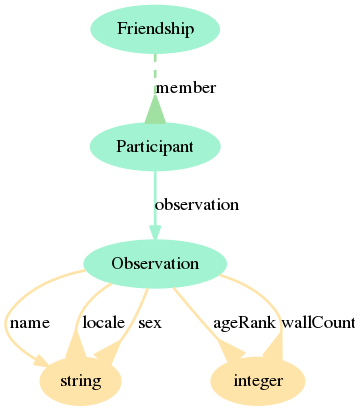
\includegraphics[width=0.5\textwidth]{../ontologies/facebook-legacy-AntonioAnzoategui18022013Friendship.ttl/draw}
    \caption{A diagram of the core structure that yields the friendship networks
    of the Facebook snapshots. A green edge denotes an OWL existential class restriction; an inverted nip denotes an OWL universal class restriction; a full (non-dashed) edge denotes an OWL functional property axiom (see Section~\ref{sont}). Further information and complete diagrams for each provenance are available in the Supporting Information document.}\label{dia}
\end{figure}

\subsection{SPARQL queries}\label{queries}
There are numerous useful and general purpose SPARQL queries to be performed against LOSD.
In this section, a selection of some of the most basic queries are made available due to their potential to be varied.
All queries assume the preamble \textttt{PREFIX po: <http://purl.org/socialparticipation/po/>}.
\begin{itemize}
  \item Retrieve the number of participants:
\begin{lstlisting}[language=spq]
SELECT (COUNT(DISTINCT ?author) as ?c) WHERE {
  ?author a po:Participant . 
}
\end{lstlisting}
  \item Retrieve the number of relations, be them interactions or
      friendships:
\begin{lstlisting}[language=spq]
SELECT (COUNT(?interaction) as ?c) WHERE {
  { ?interaction a po:Friendship } UNION { ?interaction a po:Interaction }
  UNION { ?interaction po:retweetOf ?message }
  UNION { ?interaction po:replyTo ?message }
  UNION { ?interaction po:directedTo ?participant }
}
\end{lstlisting}
            \item Retrieve all text produced by a specific user with URI \textttt{user\_uri}:
\begin{lstlisting}[language=spq]
SELECT (CONCAT(?text) as ?texts) WHERE {
  ?activity po:author <user_uri> . ?activity po:text ?text .
}
\end{lstlisting}
  \item List 1000 users (URIs and names) with the most friendships and the number of
      friendships in descending order by the number of friendships:
\begin{lstlisting}[language=spq]
SELECT DISTINCT ?participant (COUNT(?friendship) as ?c) WHERE {
  ?friendship a po:Friendship . ?friendship po:member ?participant . 
} ORDER BY DESC(?c) LIMIT 1000
\end{lstlisting}
  \item Retrieve text messages with the word ``crucial'' (case insensitive):
\begin{lstlisting}[language=spq]
SELECT ?text WHERE { 
  ?activity po:text ?text . FILTER regex(?text, 'crucial', 'i')
}
\end{lstlisting}
  \item List participants and respective full names whose name has the substring ``Amanda'':
\begin{lstlisting}[language=spq]
SELECT DISTINCT ?participant ?name WHERE {
  ?participant po:observation ?obs . ?obs po:name ?name .
  FILTER regex(?name, 'Amanda', 'i') 
}
\end{lstlisting}
  \item Return all pairs of friends of a participant (with URI \textttt{participant\_uri}) which are friends themselves:
\begin{lstlisting}[language=spq]
SELECT DISTINCT ?friend1 ?friend2 WHERE {
  ?friendship1 po:member <participant_uri> . ?friendship1 po:member ?friend1 .
  ?friendship2 po:member <participant_uri> . ?friendship2 po:member ?friend2 .
  ?friendship3 po:member ?friend1 . ?friendship3 po:member ?friend2 .
}
\end{lstlisting}
  \item Return all interactions from replies in a snapshot:
\begin{lstlisting}[language=spq]
SELECT ?from ?to WHERE {
  ?message1 po:snapshot <snapshot_uri> .  ?message2 po:replyTo ?message1 .
  ?message1 po:author ?from .  ?message2 po:author ?to .
}
\end{lstlisting}
\end{itemize}

\subsubsection{Obtaining the networks}\label{snet}
A complex network $N=(n,l,m)$ may be regarded essentially as
a set of nodes $n$, a set of links $l$ that related the nodes,
and metadata $m$ such as node and link weights, text related to the nodes, etc.
This section presents queries for obtaining networks using LOSD
which are promptly envisioned by the authors.
Many other networks may be obtained because the criteria that entail
links, and restrains in the set of nodes and of links,
are determined by the research or application being developed.
Furthermore, we do not focus here on multilayer networks (e.g. bipartite networks), or on multigraphs (or muldimensional networks), i.e. on networks with more than one type of node or of link.
Here is a list with short descriptions of the networks and the corresponding SPARQL queries:
\begin{itemize}
  \item Overall facebook friendship network available in LOSD:
\begin{lstlisting}[language=spq]
SELECT ?a1 ?a2 WHERE { 
  ?f a po:Friendship .  ?f po:member ?a1 . ?f po:member ?a2 .
}
\end{lstlisting}\vspace{-0.2cm}
  \item Overall facebook friendship network derived only from ego networks:
\begin{lstlisting}[language=spq]
SELECT ?a1 ?a2 WHERE { 
  ?f a po:Friendship . ?f po:snapshot ?s . ?s po:isEgo True .
  ?f po:member ?a1 . ?f po:member ?a2 .
}
\end{lstlisting}\vspace{-0.2cm}
  \item Overall facebook interaction network available in LOSD:
\begin{lstlisting}[language=spq]
SELECT ?a1 ?a2 WHERE { 
  ?f a po:Interaction .
  ?f po:interactionFrom ?a1 . ?f po:interactionTo ?a2 .
}
\end{lstlisting}\vspace{-0.2cm}
  \item Email interaction network for email list shapshot with URI \verb|http://xxxx|, with the all (preliminarily cleaned) text related to each message (node atribute):
\begin{lstlisting}[language=spq]
SELECT ?a1 ?a2 ?t1 ?t2 WHERE { 
  ?m po:snapshot <http://xxxx> . ?m a po:EmailMessage .
  ?m po:author ?a1 . ?m po:replyTo ?m2 . ?m2 po:author ?a2 .
  ?m po:cleanText ?t1 . ?m2 po:cleanText ?t2 .
}
\end{lstlisting}\vspace{-0.2cm}
  \item IRC users related by messages directed to each other, and the text of each message (link attribute):
\begin{lstlisting}[language=spq]
SELECT ?a1 ?a2 ?t WHERE { 
  ?m a po:IRCMessage .  ?m po:author ?a1 . ?m po:directedTo ?a2 .
  ?m po:cleanText ?t .
}
\end{lstlisting}\vspace{-0.2cm}
  \item Twitter users related by retweets:
\begin{lstlisting}[language=spq]
SELECT ?a1 ?a2 WHERE { 
  ?m1 po:retweetOf ?m2 . ?m1 po:author ?a1 . ?m2 po:author ?a2 .
}
\end{lstlisting}\vspace{-0.2cm}
  \item Twitter users related by user mentions and the text of the tweets:
\begin{lstlisting}[language=spq]
SELECT ?a1 ?a2 ?t WHERE { 
  ?m a po:Tweet . ?m po:author ?a1 . ?m po:userMention ?a2 .
  ?m po:text ?t .
}
\end{lstlisting}\vspace{-0.2cm}
  \item Friendship network from ParticipaBR, with the date when each frienship was established:
\begin{lstlisting}[language=spq]
SELECT ?a1 ?a2 ?d WHERE { 
  ?s po:shapshotID 'participabr-legacy' . ?f po:snapshot ?s .
  ?f a po:Friendship . 
  ?f po:member ?a1 . ?f po:member ?a2 . ?f po:createdAt ?d .
}
\end{lstlisting}\vspace{-0.2cm}
  \item Interaction network from ParticipaBR obtained by comments on articles:
\begin{lstlisting}[language=spq]
SELECT ?a1 ?a2 WHERE { 
  ?s po:shapshotID 'participabr-legacy' . ?a po:snapshot ?s .
  ?a a po:Article .
  ?a po:author ?a1 . ?c po:article ?a . ?c po:author ?a2 .
}
\end{lstlisting}\vspace{-0.2cm}
  \item Interaction network from ParticipaBR obtained by comments and votes on comments:
\begin{lstlisting}[language=spq]
SELECT ?a1 ?a2 WHERE { 
  ?s po:shapshotID 'participabr-legacy' . ?c po:snapshot ?s .
  ?c a po:Comment .  ?c po:author ?a1 .
  { ?v a po:Vote . ?v po:reference ?c . ?v po:author ?a2 .
  } UNION {
    ?c2 a po:Comment . ?c2 po:replyTo ?c . ?c2 po:author ?a2 .
  }
}
\end{lstlisting}\vspace{-0.2cm}
  \item Interaction network from Cidade Democrática obtained by comments on Topics:
\begin{lstlisting}[language=spq]
SELECT ?a1 ?a2 WHERE { 
  ?s po:shapshotID 'cidadedemocratica-legacy' . ?t po:snapshot ?s .
  ?t a po:Topic .  ?t po:author ?a1 .
  ?c a po:Comment . ?c po:topic ?t . ?c po:author ?a2 .
}
\end{lstlisting}\vspace{-0.2cm}
  \item AA users, related by AA session validations:
\begin{lstlisting}[language=spq]
SELECT ?a1 ?a2 WHERE { 
  ?s po:author ?a1 . ?s po:checkParticipant ?a2 .
}
\end{lstlisting}\vspace{-0.2cm}
\end{itemize}

This is not an exaustive list.
For example, other instances which are related in LOSD, and have authors,
also yield valid criteria for interaciton networks.
For a less canonical example for obtaining networks, links may be derived from sufficiently similar vocabulary used by participants, or from activity with sufficiently similar dates, which yield networks which are not interaction or friendship networks.
Figure~\ref{fnet} describes most often criteria used to obtain social networks.
% mk figure with two participants and their relation though response, retweet, or friendship TTM

\begin{figure}[H]
    \centering
    \includegraphics[width=0.5\textwidth]{../misc/netSynth____}
    \caption{Most usual paradigm for considering social networks:
    actors (i.e. participants, authors) are linked through interactions
    (e.g. replies, likes, comments)
    or relations (e.g. friendships, similar activity patterns).}\label{fnet}
\end{figure}

\subsection{Data access}\label{sac}
We highly encourage interested parties to take advantage of the API at \url{https://apidocs.data.world/toolkit/api}.
The user responsible for LOSD has id ``rfabbri'' and the dataset id is ``linked-open-social-data''.
For making use of the API, and exploiting further services provided by the platform (such as integrations with data analysis software), the researcher needs to register in Data.World, which is fast and free, and facilitates assistance by the platform maintainers.
Anonynous (not authenticated) SPARQL queries may be performed using the endpoint at: \url{https://rfabbri.linked.data.world/sparql/linked-open-social-data}, kindly provided by the Data.World staff.

\subsection{Example network}\label{sex}
Figure~\ref{caleb} exemplifies a network obtained through a SPARQL query made to LOSD. The nodes are colored and sized according to network metrics, as explained in the caption. With \te{http://purl.org/socialparticipation/po/Snapshot\#facebook-legacy-CalebLuporini13042013} as the \te{snaphot\_uri}, the query performed to find the network is:
\begin{lstlisting}[language=spq]
PREFIX po: <http://purl.org/socialparticipation/po/>
SELECT ?a1 ?a2 WHERE {
  ?f a po:Friendship . ?f po:snapshot <snapshot_uri> .
  ?f po:member ?a1, ?a2 .
  FILTER(?a1 != ?a2 && ?a1 > ?a2)
}
\end{lstlisting}

\begin{figure}[H]
    \centering
    \includegraphics[width=0.8\textwidth]{../misc/caleb}
    \caption{
      A network retrieved from LOSD as described in Section~\ref{sex}.
  Nodes are colored according to clustering coefficient (greatest values are green, smallest values are pink) and their sizes are proportional to degree (number of links). The network has 1032 nodes and 24653 links, average degree of 47.77, average clustering coefficient of 0.47, diameter of 7 (greatest shortest path between nodes), etc.
    }\label{caleb}
\end{figure}

\section{Conclusions and further work}
\label{conclusions}
This article outlined LOSD, a large human online social networking dataset, with almost 32 million triples and diverse provenance.
Tools and procedures used to achieve LOSD, and fundamental queries needed to retrieve the data, were also described to the convenience of the newcommer
and for a consistent exposition.
All data is publicly available, and the scientific community now has consistent and curated data
that enables research validation, continuity, and benchmarking.
The diagrams and tables of the Supplementary document of this article
has further directions on the available structures and is an overview complement.

The authors plan on using LOSD for analyzing simple, bipartite
and dynamic (i.e. time-evolving) networks.
The research and development of data visualization interfaces using LOSD
is envisioned by the authors (FAPESP grant ).
Directly related to publications, the authors should submite a short paper
describing and exploring the data collection procedure outlined in Section~\ref{acq} and the data-driven ontology synthesis outlined in Section~\ref{ont}.
For enhancing LOSD, it should be expanded upon need or request from interested parties.
Also, software packages for LOSD data retrieval and analysis should be made available.
Routines for anonymization of LOSD data may be desired in order to preserve privacy of the participants~\cite{ieee}.
Careful linkage of LOSD classes and entities with third party data (e.g. DBPedia or other Data.World datasets) should make LOSD a five start dataset~\cite{5star}.


%%%%%%%%%%%%%%%%%%%%%%%%%%%%%%%%%%%%%%%%%%
%% optional
\supplementary{The following are available online at \linksupplementary{s1}, Figure S1: title, Table S1: title, Video S1: title.}

%%%%%%%%%%%%%%%%%%%%%%%%%%%%%%%%%%%%%%%%%%
\authorcontributions{Conceptualization, writing, formal analysis, R.F; senior supervision, final writing, O.N.O.Jr.}

%%%%%%%%%%%%%%%%%%%%%%%%%%%%%%%%%%%%%%%%%%
\funding{This research was funded by CNPq (grant 14068/2013-4) and FAPESP (grant 2017/05838-3).}

%%%%%%%%%%%%%%%%%%%%%%%%%%%%%%%%%%%%%%%%%%
\acknowledgments{
The authors acknowledge the financial support of the São Paulo State Research Foundation (FAPESP grant 2017/05838-3) and the National Council for Scientific and Technological Development (CNPq, grant 140860/2013-4).
The authors thank Data.World staff for providing the technical assistance when for providing LOSD,
for providing the authors the possibility of uploading LOSD which is above their standard size limits,
and for providing the authors and the scientific community the public query endpoint mentioned in Section~\ref{sac}.
The views expressed do not reflect the official policy or position of FAPESP, CNPq or Data.World.
The authors thank all participants in the experiments which resulted in the donation of the data they gathered as described in Section~\ref{acq}.
}
%%%%%%%%%%%%%%%%%%%%%%%%%%%%%%%%%%%%%%%%%%
\conflictsofinterest{The authors declare no conflict of interest. The funders had no role in the design of the study; in the collection, analyses, or interpretation of data; in the writing of the manuscript, or in the decision to publish the results.} 

%%%%%%%%%%%%%%%%%%%%%%%%%%%%%%%%%%%%%%%%%%
%% optional
% \appendixtitles{no} %Leave argument "no" if all appendix headings stay EMPTY (then no dot is printed after "Appendix A"). If the appendix sections contain a heading then change the argument to "yes".
% \appendix
% \section{}
% \unskip
% \subsection{}
% The appendix is an optional section that can contain details and data supplemental to the main text. For example, explanations of experimental details that would disrupt the flow of the main text, but nonetheless remain crucial to understanding and reproducing the research shown; figures of replicates for experiments of which representative data is shown in the main text can be added here if brief, or as Supplementary data. Mathematical proofs of results not central to the paper can be added as an appendix.
% 
% \section{}
% All appendix sections must be cited in the main text. In the appendixes, Figures, Tables, etc. should be labeled starting with `A', e.g., Figure A1, Figure A2, etc. 

%%%%%%%%%%%%%%%%%%%%%%%%%%%%%%%%%%%%%%%%%%
\reftitle{References}

% Please provide either the correct journal abbreviation (e.g. according to the “List of Title Word Abbreviations” http://www.issn.org/services/online-services/access-to-the-ltwa/) or the full name of the journal.
% Citations and References in Supplementary files are permitted provided that they also appear in the reference list here. 

%=====================================
% References, variant A: external bibliography
%=====================================
\externalbibliography{yes}
\bibliography{../paper}


%%%%%%%%%%%%%%%%%%%%%%%%%%%%%%%%%%%%%%%%%%
%% optional
%%%%%%%%%%%%%%%%%%%%%%%%%%%%%%%%%%%%%%%%%%
\end{document}

